% !TEX root = ../prospector.tex

\begin{figure}[t]
\centering
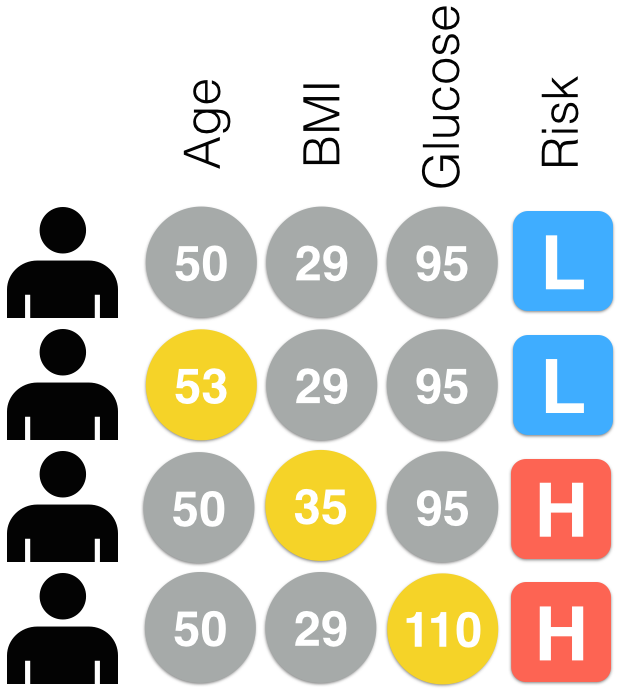
\includegraphics[width=0.3\linewidth]{prospector/local-inspection-explanation} % 0.3
\caption[Explanation of how local inspection works.]{
This illustration provides an explanation of how local inspection works.  On the top row are the patient's original feature values and the corresponding prediction.  On the bottom three rows, users changed certain values of the patient, highlighted in yellow, and such values impacted the prediction.
}
\label{figs:liexplain}
\end{figure}